\section{STM in ABS}
\label{sec:stm_abs}
In this section we give a short overview of how we apply STM in our ABS. We fundamentally follow a time-driven approach in both case-studies where the simulation is advanced by some given $\Delta t$ and in each step all agents are executed. To employ parallelism, each agent runs within its own thread and agents are executed in lock-step, synchronising between each $\Delta t$ which is controlled by the main thread. See Figure \ref{fig:stm_abs_structure} for a visualisation of our time-driven lock-step approach.

An agent thread will block until the main thread sends the next $\Delta t$ and runs the STM action atomically with the given $\Delta t$. When the STM action has been committed, the thread will send the output of the agent action to the main-thread to signal it has finished. The main thread awaits the results of all agents to collect them for output of the current step e.g. visualisation or writing to a file.

As will be described in subsequent sesctions, central to both case-studies is an environment which is shared between the agents using a \textit{TVar} or \textit{TArray} primitive through which the agents communicate concurrently with each other. To get the environment in each step visualisation purposes, the main thread can access the \textit{TVar} and \textit{TArray} as well. 

\begin{figure}
	\centering
	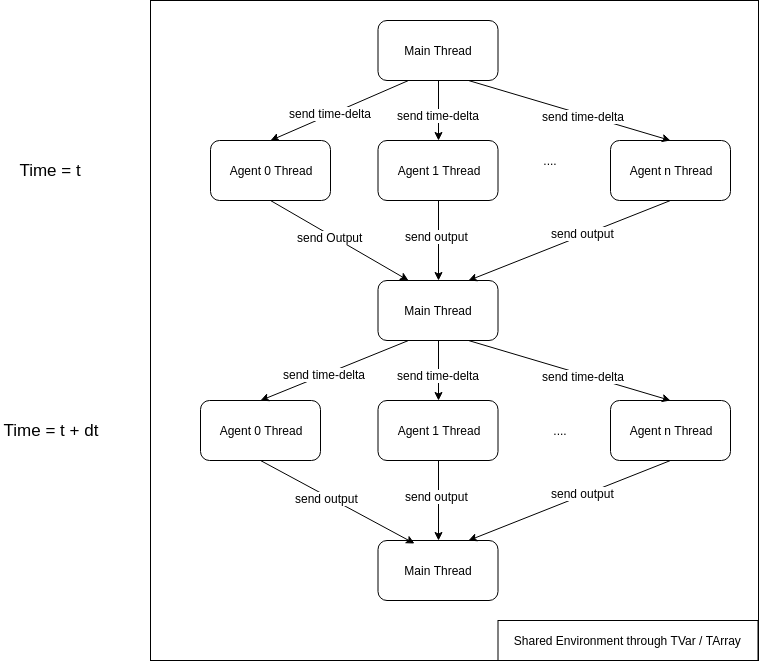
\includegraphics[width=0.6\textwidth, angle=0]{./fig/dia/stm_abs.png}
	\caption{Diagram of the parallel time-driven lock-step approach.}
	\label{fig:stm_abs_structure}
\end{figure}